\subsection{Zbiór "Glass"}
    \begin{figure}[H]
        \center
        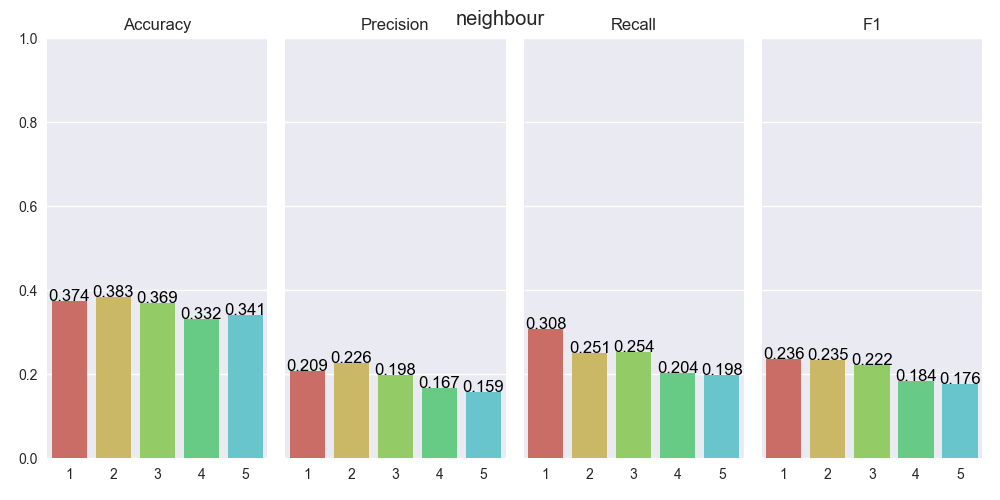
\includegraphics[width=\textwidth]{resources/plots/glass_KFold_neighbour.png}
        \caption{Wykres wartości miar dla zbioru "Glass" dla różnej liczby sąsiadów (kroswalidacja zwykła).}
    \end{figure}

    \begin{figure}[H]
        \center
        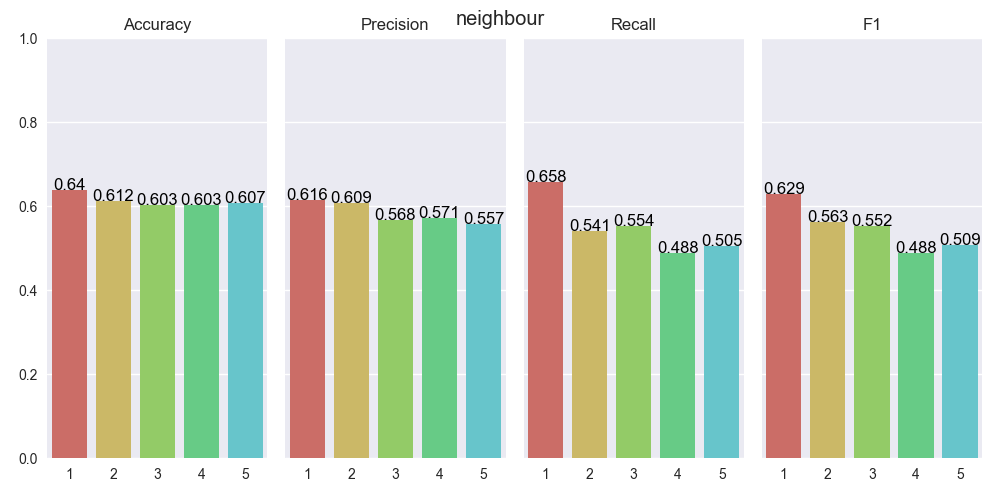
\includegraphics[width=\textwidth]{resources/plots/glass_StratifiedKFold_neighbour.png}
        \caption{Wykres wartości miar dla zbioru "Glass" dla różnej liczby sąsiadów (kroswalidacja stratyfikowana).}
    \end{figure}

    \pagebreak

    \begin{figure}[H]
        \center
        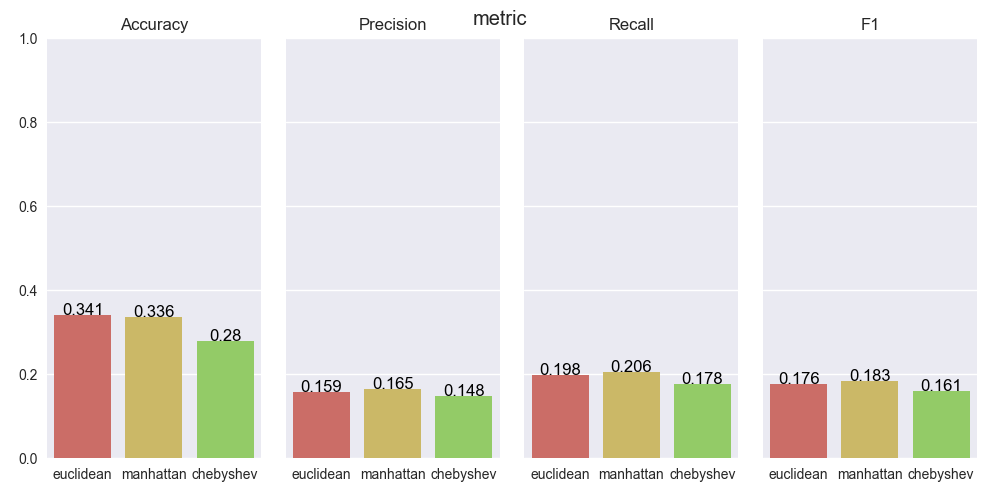
\includegraphics[width=\textwidth]{resources/plots/glass_KFold_metric.png}
        \caption{Wykres wartości miar dla zbioru "Glass" dla różnych metryk odległości (kroswalidacja zwykła).}
    \end{figure}

    \begin{figure}[H]
        \center
        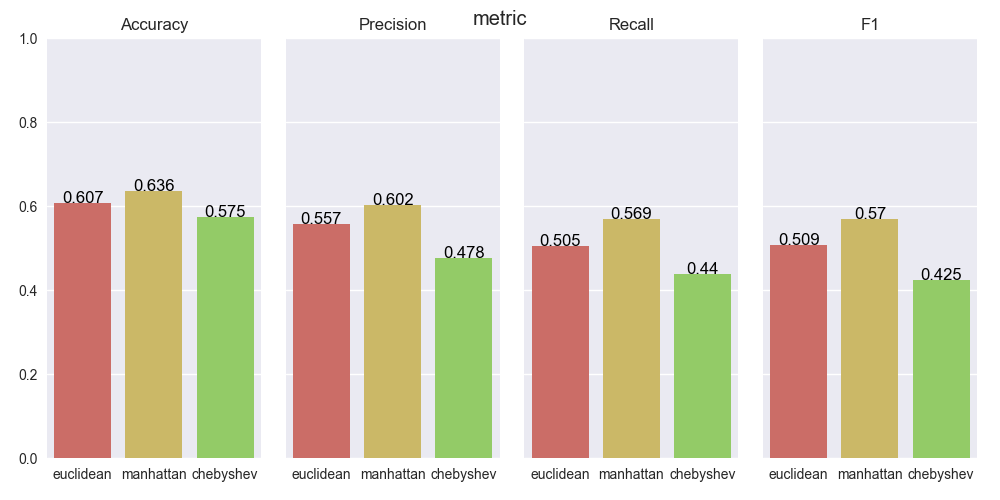
\includegraphics[width=\textwidth]{resources/plots/glass_StratifiedKFold_metric.png}
        \caption{Wykres wartości miar dla zbioru "Glass" dla różnych metryk odległości (kroswalidacja stratyfikowana).}
    \end{figure}

    \pagebreak

    \begin{figure}[H]
        \center
        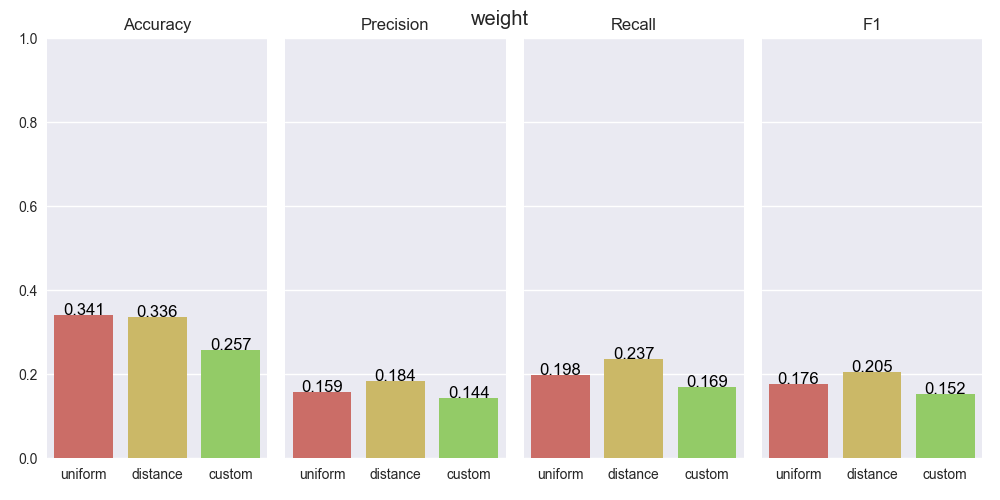
\includegraphics[width=\textwidth]{resources/plots/glass_KFold_weight.png}
        \caption{Wykres wartości miar dla zbioru "Glass" dla różnych sposobów głosowania (kroswalidacja zwykła).}
    \end{figure}

    \begin{figure}[H]
        \center
        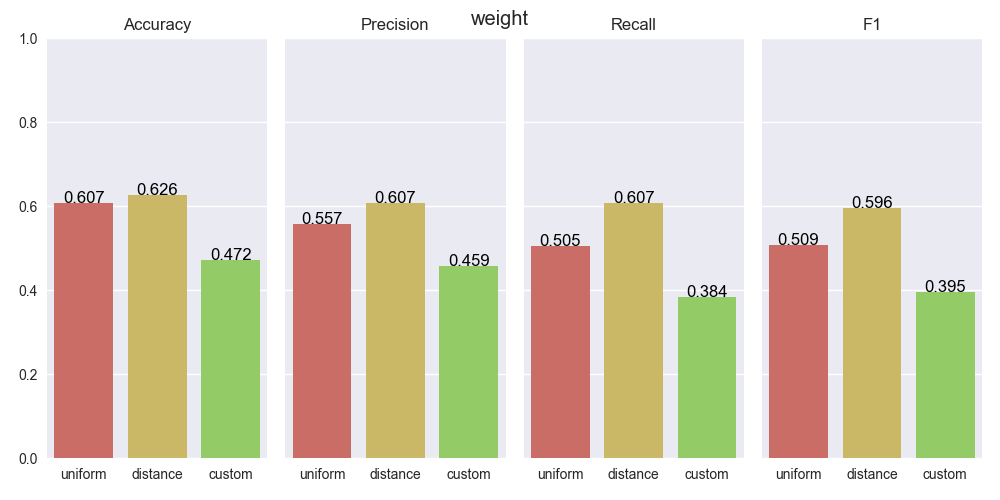
\includegraphics[width=\textwidth]{resources/plots/glass_StratifiedKFold_weight.png}
        \caption{Wykres wartości miar dla zbioru "Glass" dla różnych sposobów głosowania (kroswalidacja stratyfikowana).}
    \end{figure}
